\setcounter{page}{1}
\pagenumbering{Roman}

\section{Appendix}

% Listado de apartados que son demasiado extensos para incluir en la memoria y tienen un carácter autocontenido (por ejemplo, manuales de usuario, manuales de instalación, etc.)
 
% Dependiendo del tipo de trabajo, es posible que no sea necesario añadir ningún anexo.

\subsection*{Appendix A: RNA motifs employed in this work, as seen in \cite{dolcemascolo_2022} (in \texttt{.fasta} format)}\label{appendix_A}
\addcontentsline{toc}{subsection}{Appendix A: RNA motifs employed in this work, as seen in \cite{dolcemascolo_2022} (in \texttt{.fasta} format)}

\lstinputlisting{assets/motifs.fasta}

\subsection*{Appendix B: \texttt{Python} script to treat the RNA motifs}\label{appendix_B}
\addcontentsline{toc}{subsection}{Appendix B: \texttt{Python} script to treat the RNA motifs}

\lstinputlisting[language=Python]{assets/motifs_treatment.py}

\subsection*{Appendix C: \texttt{Python} script to relabel \texttt{HIS} residues for their corresponding \texttt{AMBER94} compatible residues}\label{appendix_C}
\addcontentsline{toc}{subsection}{Appendix C: \texttt{Python} script to relabel \texttt{HIS} residues for their corresponding \texttt{AMBER94} compatible residues}\label{appendix_C}

\lstinputlisting[language=Python]{assets/fixHIS.py}

% \subsection*{Anexo A: Script de \texttt{Python} para la mitigación de los tags \texttt{R} en los ficheros \texttt{.pdb} de los RNAs}\label{anexo_A}
% \addcontentsline{toc}{subsection}{Anexo A: Script de \texttt{Python} para la mitigación de los tags \texttt{R} en los ficheros \texttt{.pdb} de los RNAs}

% \lstinputlisting[language=Python]{assets/manipulateRNA.py}

% \subsection*{Anexo B: Script de \texttt{Python} para la recuperación de los tags \texttt{R} en los ficheros \texttt{.pdb} de los RNAs}\label{anexo_B}
% \addcontentsline{toc}{subsection}{Anexo B: Script de \texttt{Python} para la recuperación de los tags \texttt{R} en los ficheros \texttt{.pdb} de los RNAs}

% \lstinputlisting[language=Python]{assets/manipulateRNAagain.py}

% \subsection*{Anexo C: Script de \texttt{Python} para eliminar grupos hydroxilos en los extremos 3' y 5'}\label{anexo_C}
% \addcontentsline{toc}{subsection}{Anexo C: Script de \texttt{Python} para eliminar grupos hydroxilos en los extremos 3' y 5'}

% \lstinputlisting[language=Python]{assets/removeEnds.py}



% \subsection*{Anexo E: Visualización de los 10 mejores modelos de docking entre MSI-1 y el RNA original (\textit{wild type})}\label{anexo_E}
% \addcontentsline{toc}{subsection}{Anexo E: Visualización de los 10 mejores modelos de docking entre MSI-1 y el RNA original (\textit{wild type})}

% \begin{center}
%     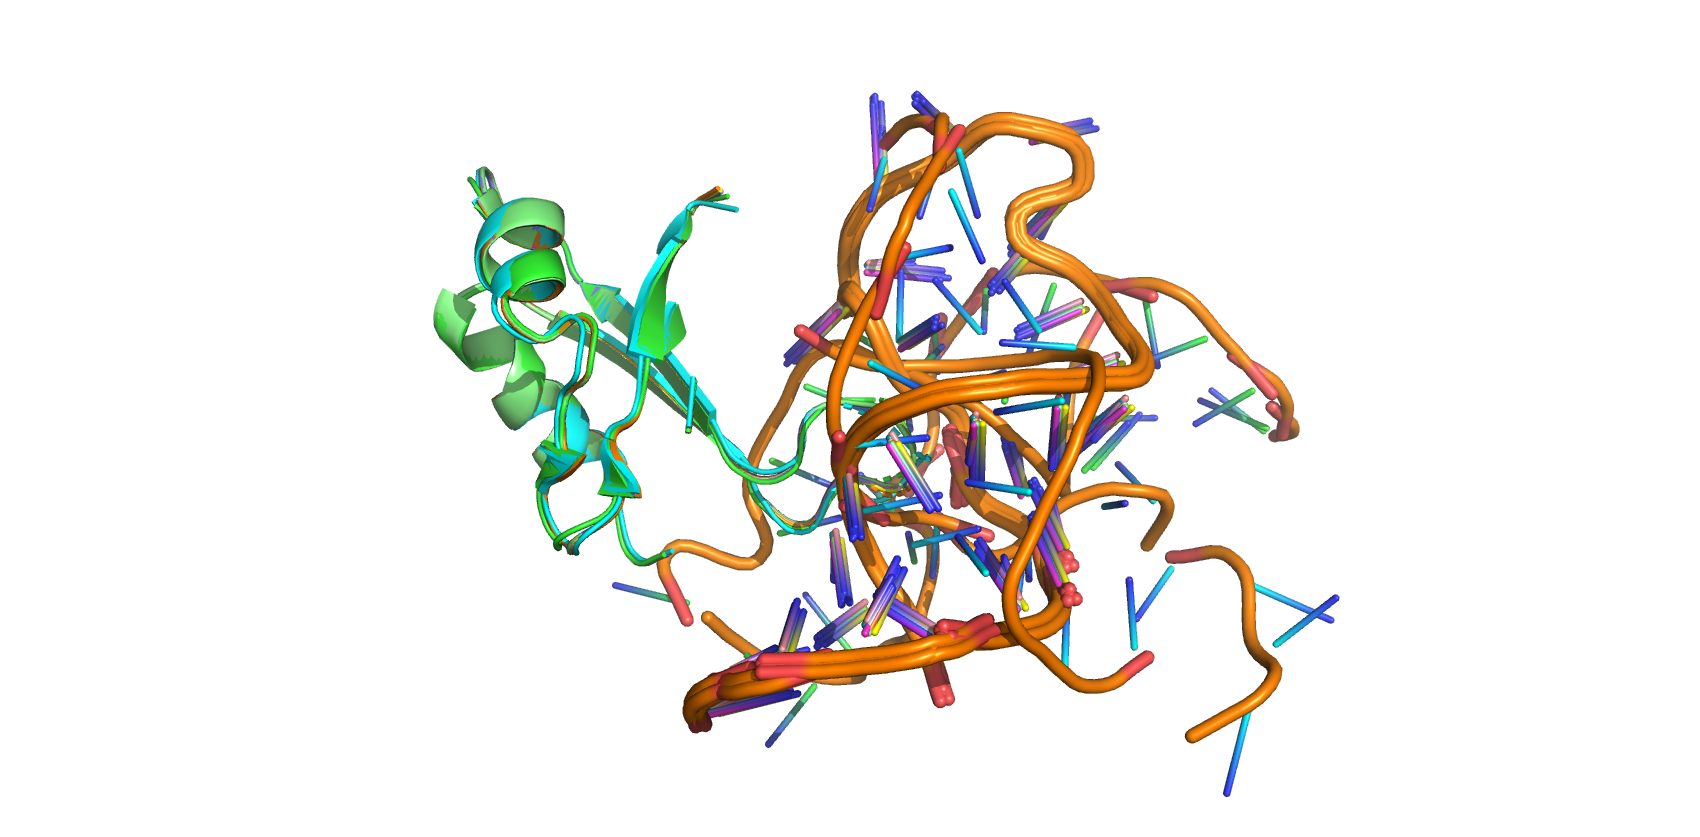
\includegraphics[width=\linewidth]{assets/RMM1_orig_ALL.png}
% \end{center}

% Podemos observar que los modelos difieren entre sí. En los subsiguientes anexos, estos modelos serán desglosados. Visualizado con \href{https://pymol.org/2/}{\texttt{Pymol}}.

% \subsection*{Anexo F: Visualización del mejor modelo de docking entre MSI-1 y el RNA original (\textit{wild type})}\label{anexo_F}
% \addcontentsline{toc}{subsection}{Anexo F: Visualización del mejor modelo de docking entre MSI-1 y el RNA original (\textit{wild type})}

% \begin{center}
%     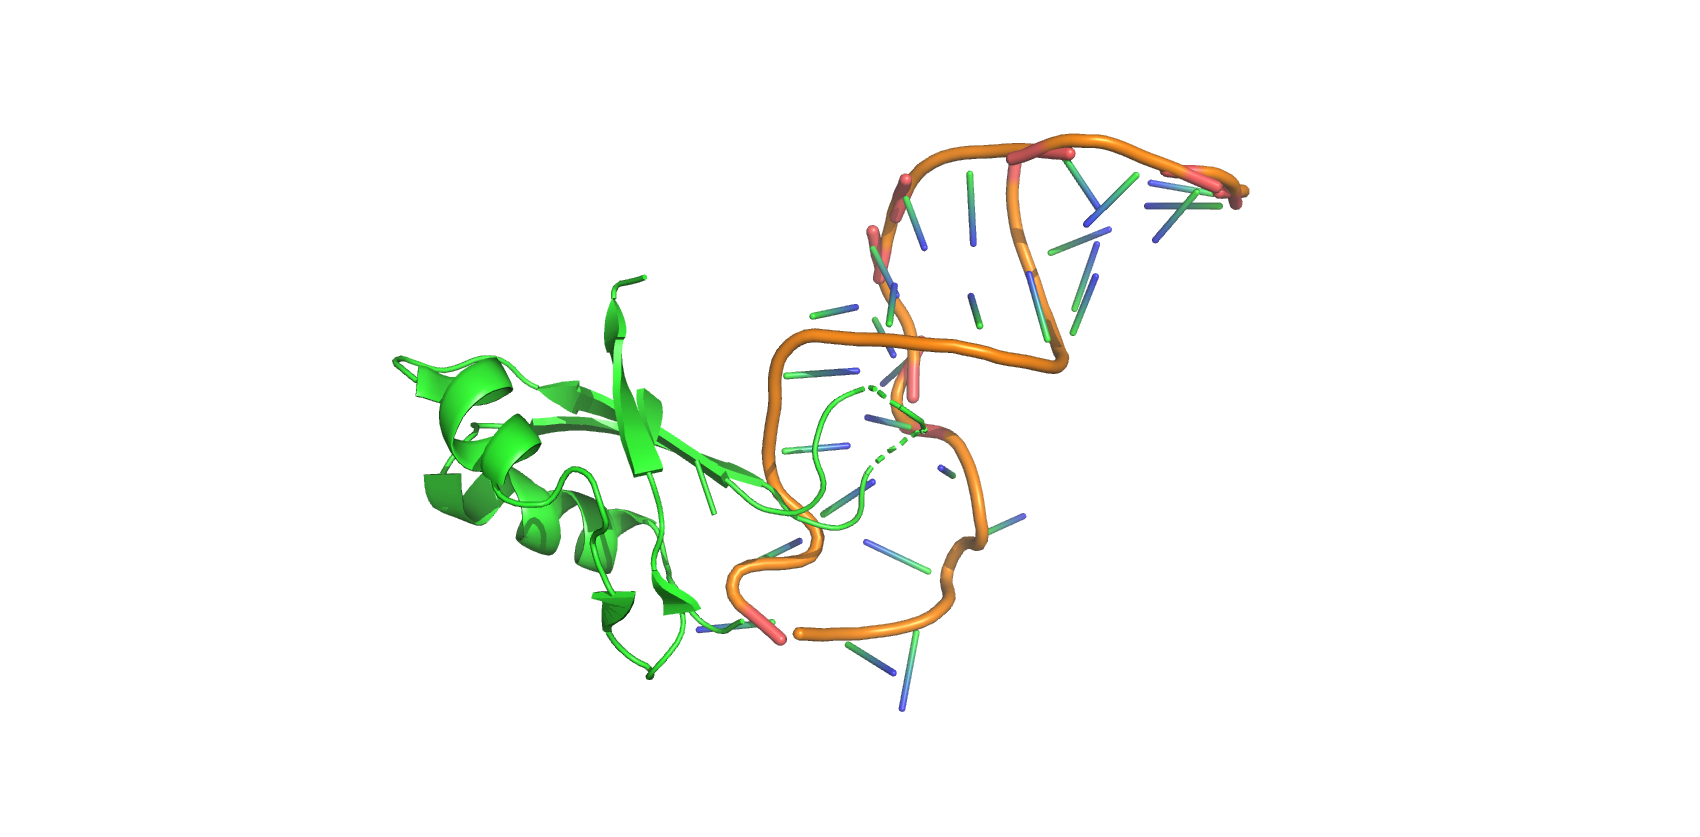
\includegraphics[width=\linewidth]{assets/RMM1_orig_top0.png}
% \end{center}

% Visualizado con \href{https://pymol.org/2/}{\texttt{Pymol}}.

% \subsection*{Anexo G: Visualización del segundo mejor modelo de docking entre MSI-1 y el RNA original (\textit{wild type})}\label{anexo_G}
% \addcontentsline{toc}{subsection}{Anexo G: Visualización del segundo mejor modelo de docking entre MSI-1 y el RNA original (\textit{wild type})}

% \begin{center}
%     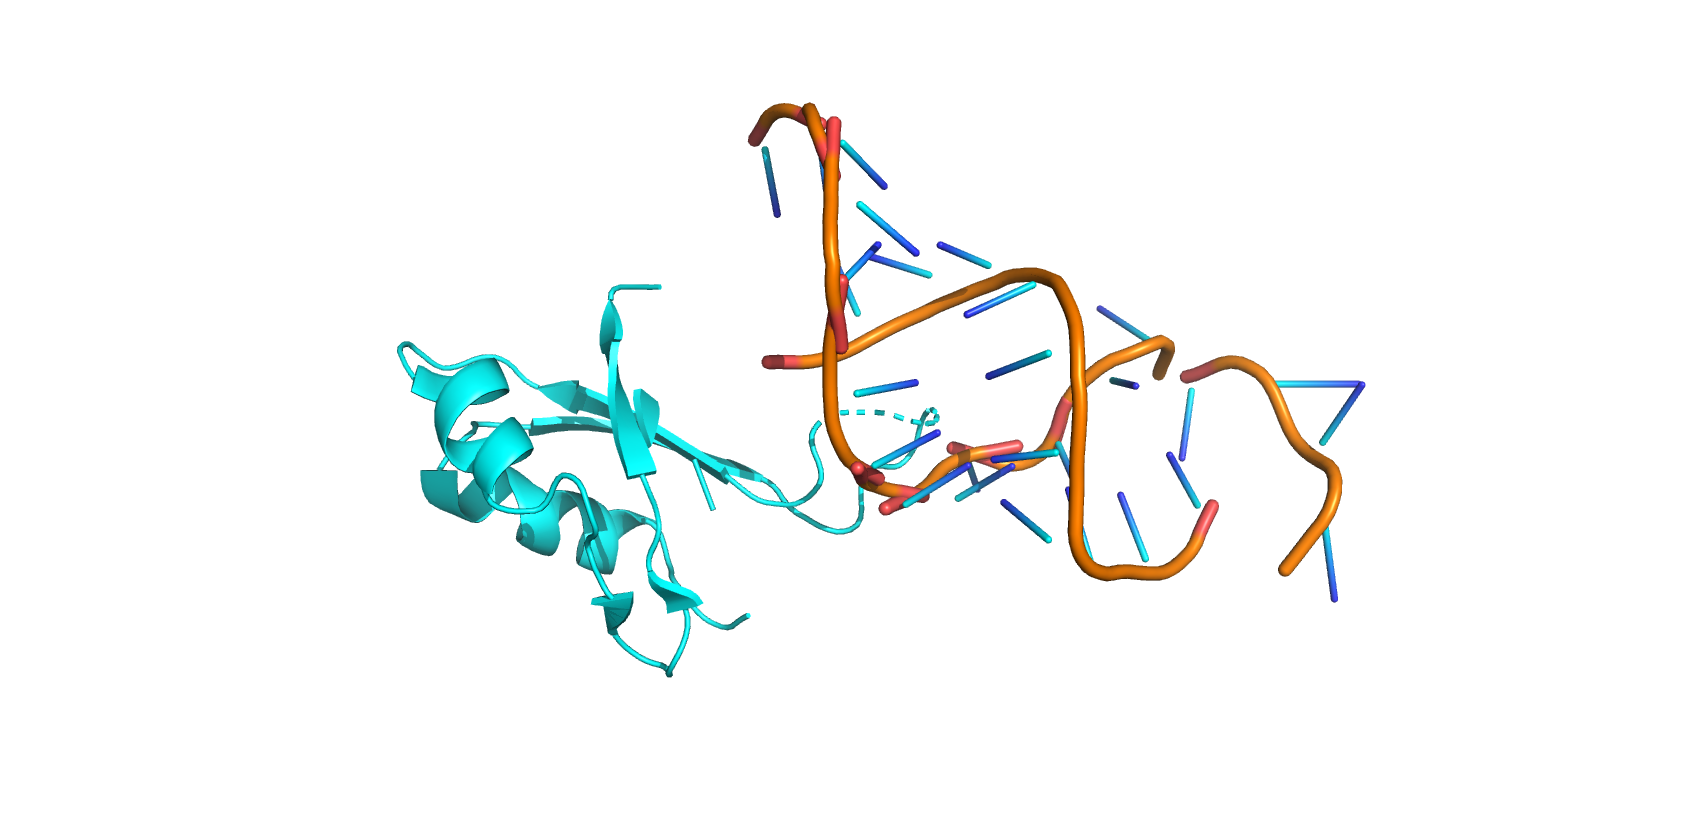
\includegraphics[width=\linewidth]{assets/RMM1_orig_top1.png}
% \end{center}

% Visualizado con \href{https://pymol.org/2/}{\texttt{Pymol}}.

% \subsection*{Anexo H: Visualización del tercer al décimo mejores modelos de docking entre MSI-1 y el RNA original (\textit{wild type})}\label{anexo_H}
% \addcontentsline{toc}{subsection}{Anexo H: Visualización del tercer al décimo mejores modelos de docking entre MSI-1 y el RNA original (\textit{wild type})}

% \begin{center}
%     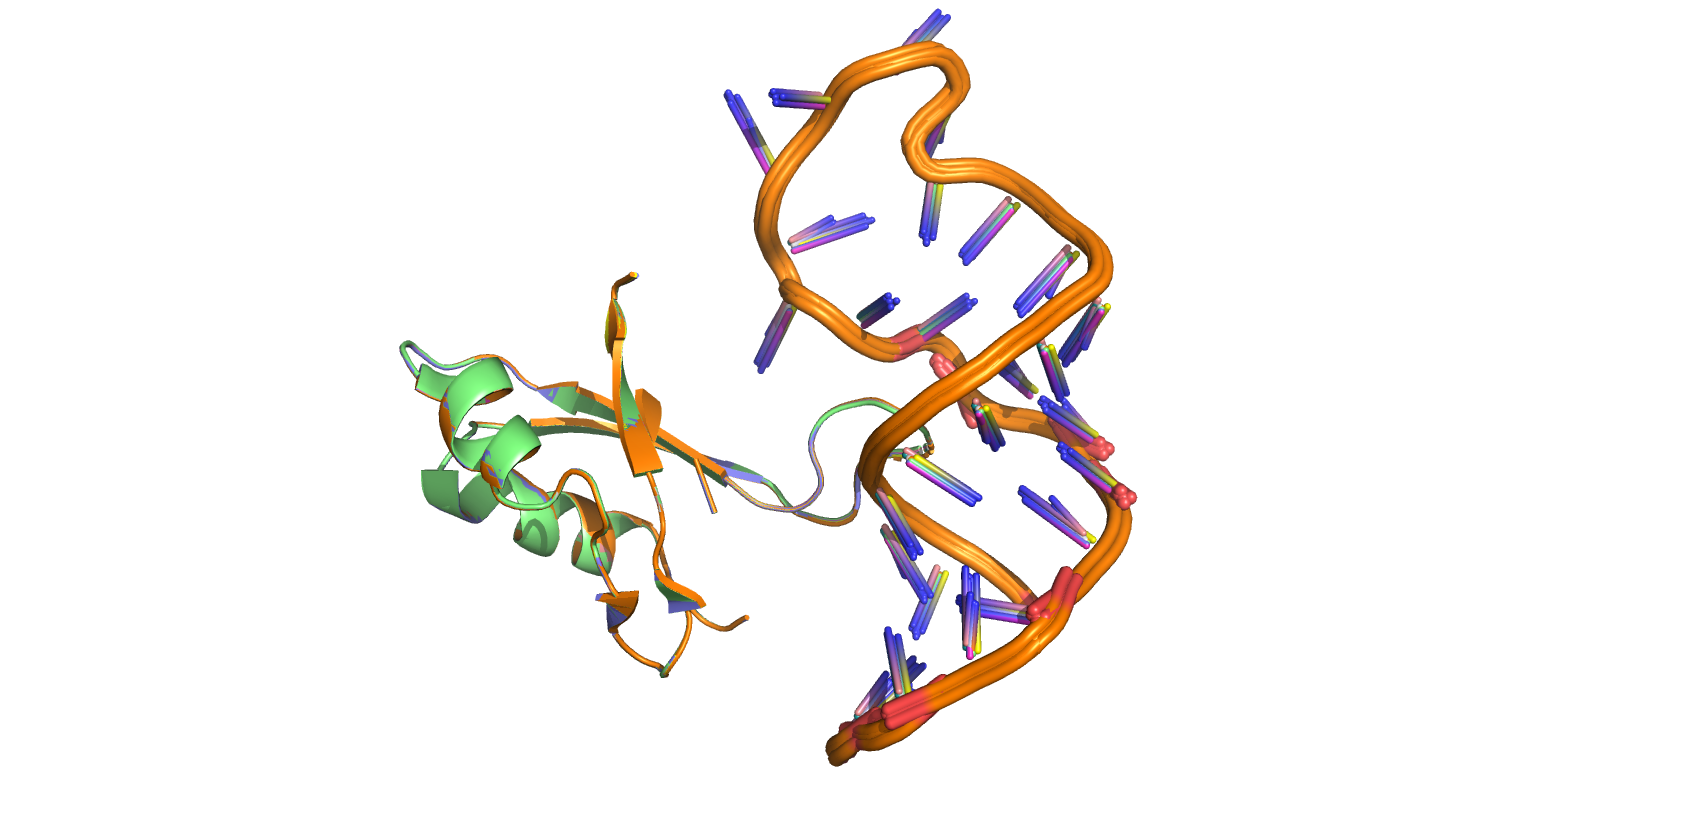
\includegraphics[width=\linewidth]{assets/RMM1_orig_2to8.png}
% \end{center}

% Podemos observar que estos modelos son casi equivalentes. Visualizado con \href{https://pymol.org/2/}{\texttt{Pymol}}.

% \subsection*{Anexo I: Visualización de los 10 mejores modelos de docking entre MSI-1 y el RNA mutante 1}\label{anexo_I}
% \addcontentsline{toc}{subsection}{Anexo I: Visualización de los 10 mejores modelos de docking entre MSI-1 y el RNA mutante 1}

% \begin{center}
%     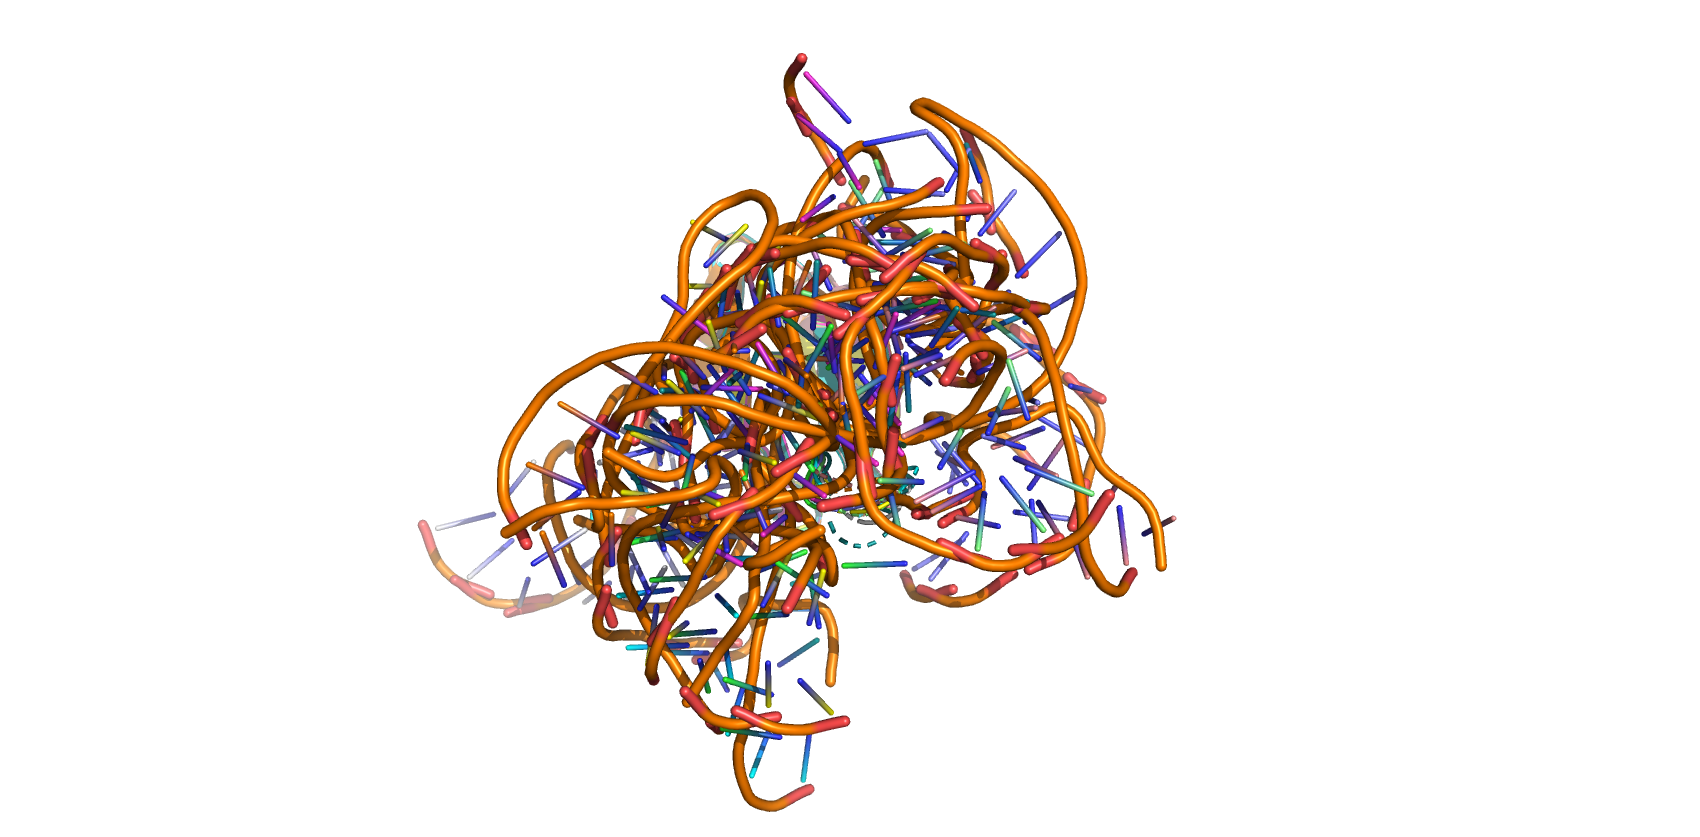
\includegraphics[width=0.9\linewidth]{assets/RMM1_mut1_ALL.png}
% \end{center}

% Podemos observar que los modelos difieren muchísimo entre sí. Parece ser que la mutación desestabiliza la interacción.  Visualizado con \href{https://pymol.org/2/}{\texttt{Pymol}}.

% \subsection*{Anexo J: Visualización de los 10 mejores modelos de docking entre MSI-1 y el RNA mutante 2}\label{anexo_J}
% \addcontentsline{toc}{subsection}{Anexo J: Visualización de los 10 mejores modelos de docking entre MSI-1 y el RNA mutante 2}

% \begin{center}
%     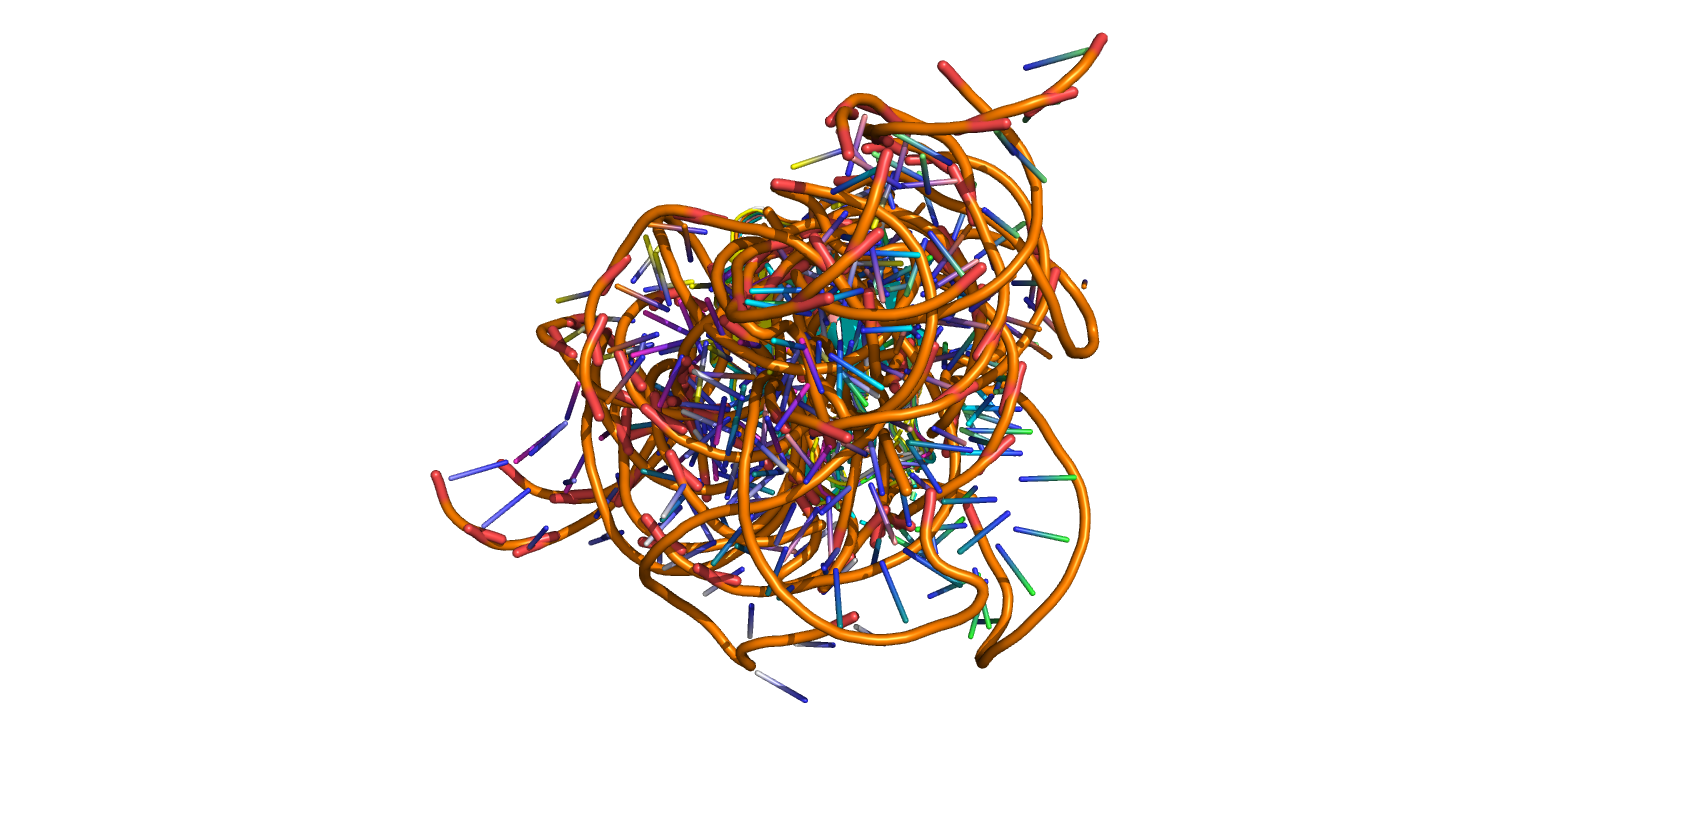
\includegraphics[width=0.9\linewidth]{assets/RMM1_mut2_ALL.png}
% \end{center}

% Podemos observar que los modelos difieren muchísimo entre sí. Parece ser que la mutación desestabiliza la interacción.  Visualizado con \href{https://pymol.org/2/}{\texttt{Pymol}}.

% \subsection*{Anexo K: Visualización de los 10 mejores modelos de docking entre MSI-1 y el RNA mutante 3}\label{anexo_K}
% \addcontentsline{toc}{subsection}{Anexo K: Visualización de los 10 mejores modelos de docking entre MSI-1 y el RNA mutante 3}

% \begin{center}
%     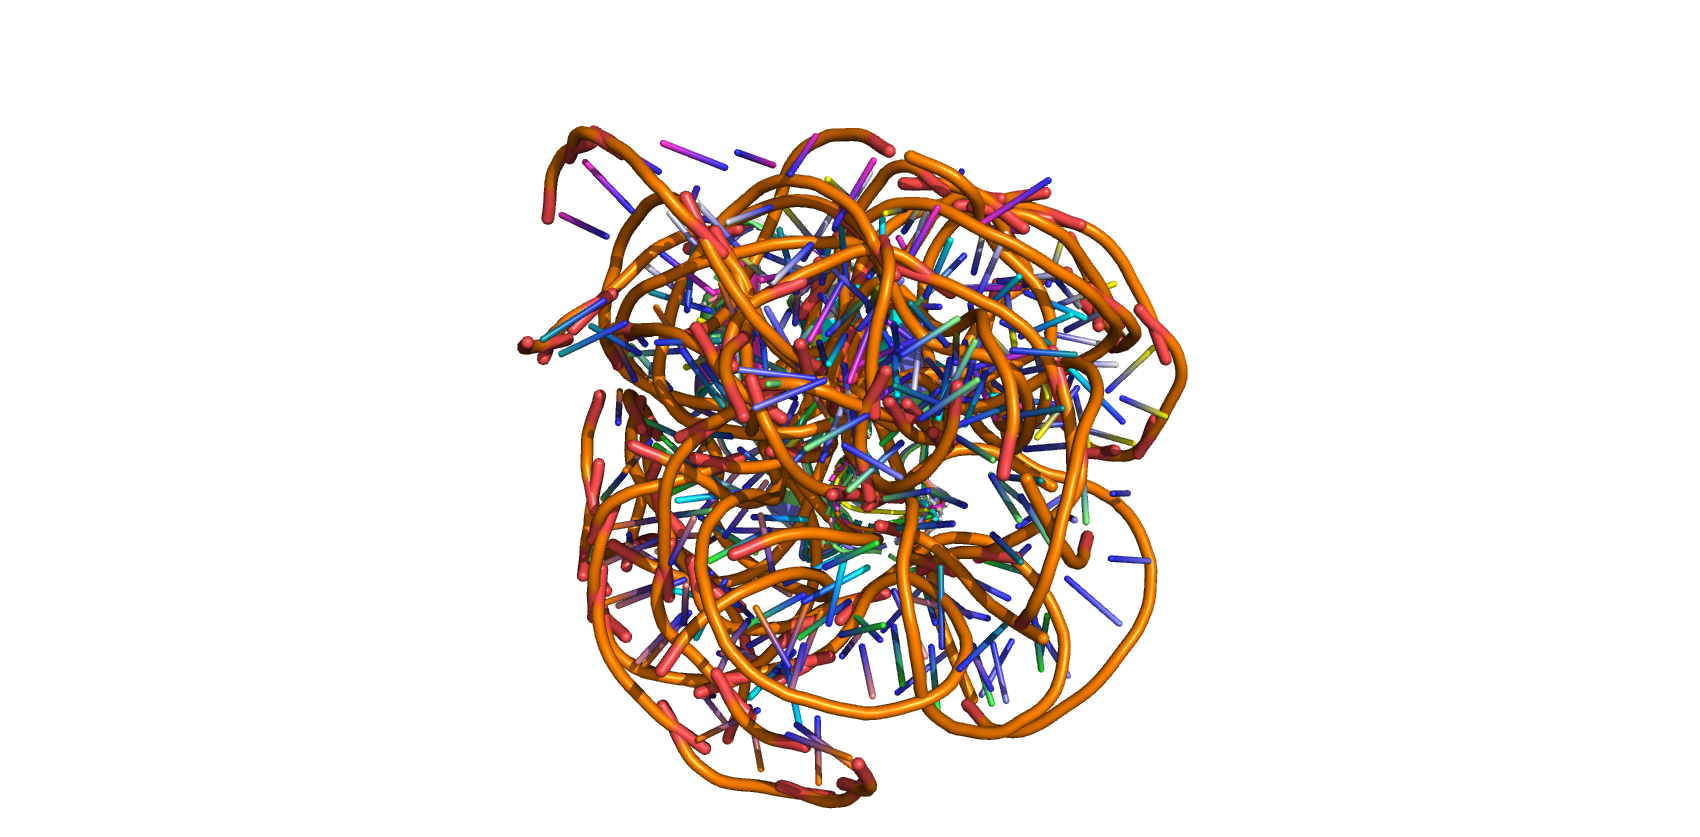
\includegraphics[width=0.9\linewidth]{assets/RMM1_mut3_ALL.png}
% \end{center}

% Podemos observar que los modelos difieren muchísimo entre sí. Parece ser que la mutación desestabiliza la interacción.  Visualizado con \href{https://pymol.org/2/}{\texttt{Pymol}}.

% \subsection*{Anexo L: Visualización de los 10 mejores modelos de docking entre MSI-1 y el RNA mutante 4}\label{anexo_L}
% \addcontentsline{toc}{subsection}{Anexo L: Visualización de los 10 mejores modelos de docking entre MSI-1 y el RNA mutante 4}

% \begin{center}
%     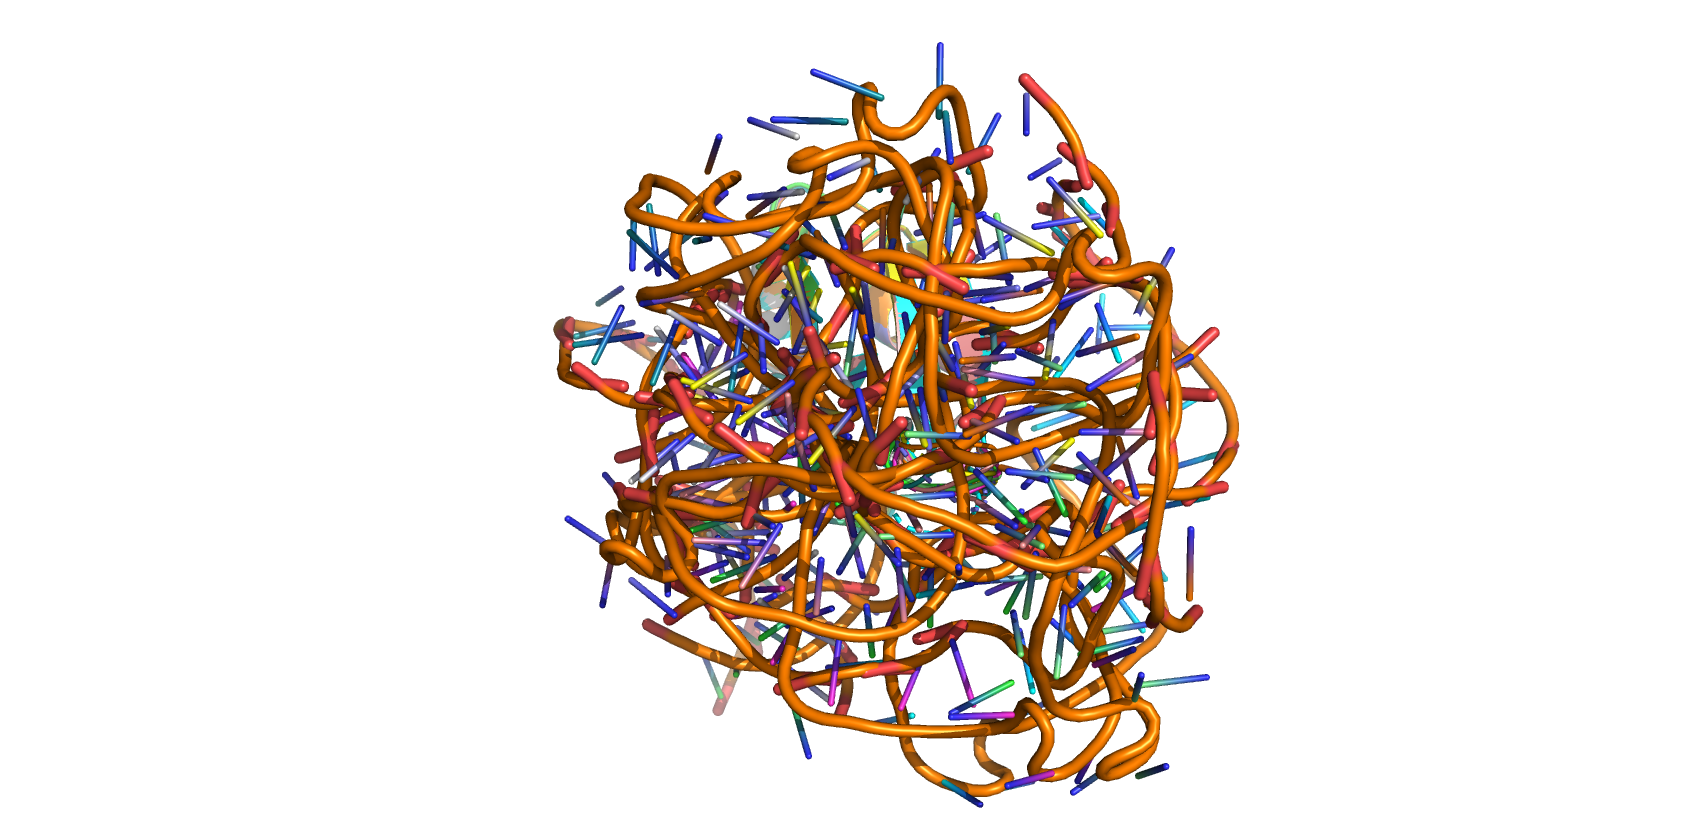
\includegraphics[width=0.9\linewidth]{assets/RMM1_mut4_ALL.png}
% \end{center}

% Podemos observar que los modelos difieren muchísimo entre sí. Parece ser que la mutación desestabiliza la interacción.  Visualizado con \href{https://pymol.org/2/}{\texttt{Pymol}}.

% \subsection*{Anexo M: Visualización de los 10 mejores modelos de docking entre MSI-1 y el RNA mutante 5}\label{anexo_M}
% \addcontentsline{toc}{subsection}{Anexo M: Visualización de los 10 mejores modelos de docking entre MSI-1 y el RNA mutante 5}

% \begin{center}
%     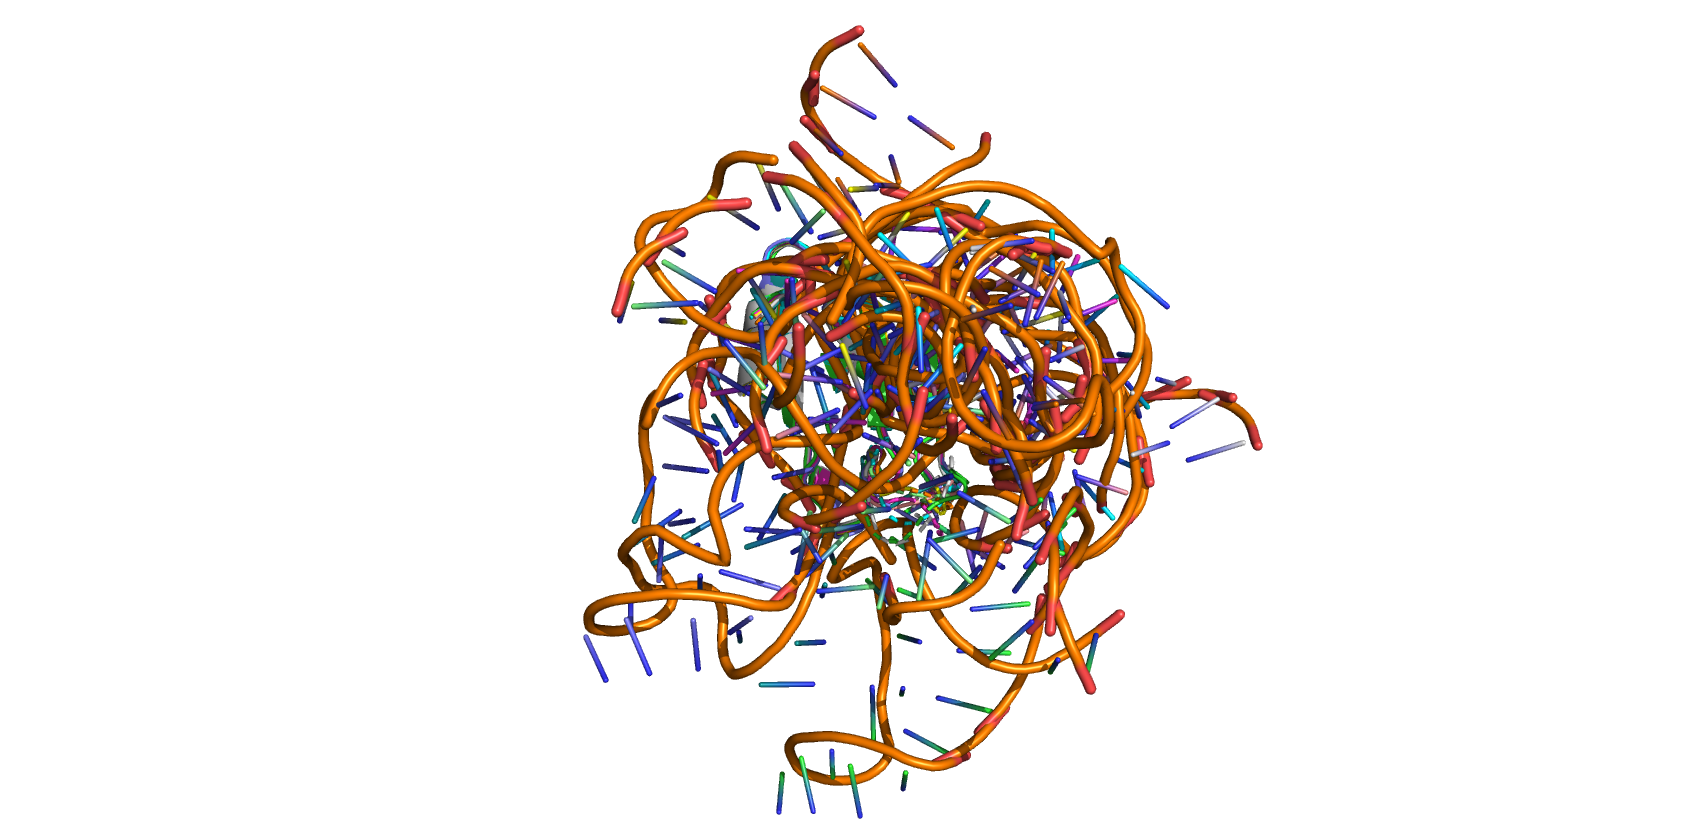
\includegraphics[width=0.9\linewidth]{assets/RMM1_mut5_ALL.png}
% \end{center}

% Podemos observar que los modelos difieren muchísimo entre sí. Parece ser que la mutación desestabiliza la interacción.  Visualizado con \href{https://pymol.org/2/}{\texttt{Pymol}}.

% \subsection*{Anexo N: Tabla de scores para los 10 mejores modelos de cada experimento de docking}\label{anexo_N}
% \addcontentsline{toc}{subsection}{Anexo N: Tabla de scores para los 10 mejores modelos de cada experimento de docking}

% \lstinputlisting{assets/allScores.table}

% \subsection*{Anexo O: Visualización de los 10 mejores modelos de docking entre MSI-1 y el RNA original en estructura lineal (sin estructura secundaria)}\label{anexo_O}
% \addcontentsline{toc}{subsection}{Anexo O: Visualización de los 10 mejores modelos de docking entre MSI-1 y el RNA original en estructura lineal (sin estructura secundaria)}

% \begin{center}
%     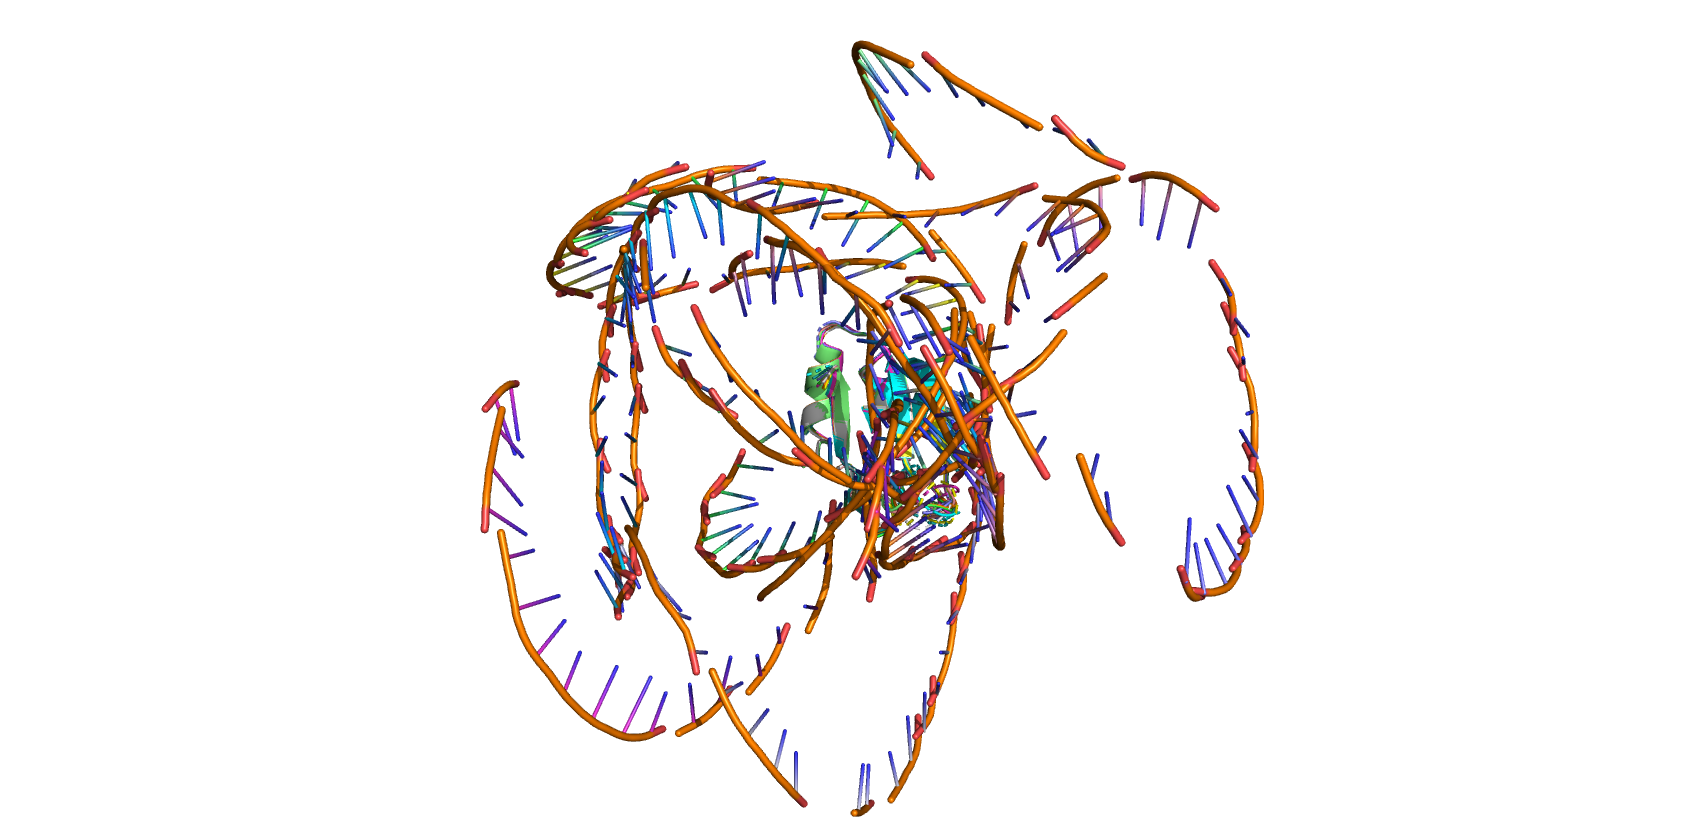
\includegraphics[width=\linewidth]{assets/linear_no_restraints.png}
% \end{center}

% Podemos observar que los modelos difieren muchísimo entre sí. En comparación con la simulación mediante el RNA con la estructura secundaria adecuada, la estructura lineal da peores resultados. Este resultado es coherente con la naturaleza, puesto que en disolución, el RNA adopta estructuras secundarias para la minimización de su energía libre de Gibbs.  Visualizado con \href{https://pymol.org/2/}{\texttt{Pymol}}.